\documentclass{article}
\oddsidemargin = 1pt
\marginparwidth = 1pt
\textwidth = 450pt
\usepackage[utf8]{inputenc}
\usepackage{graphicx}

\title{PROGETTO DEL CORSO IN430 \\ DATA PRIVACY \& FACIAL DETECTION}
\author{Simone Castellitto}
\date{November 2019}

\begin{document}

\begin{figure}
    \centering
    
\includegraphics{images/Logo_Roma_Tre.jpg}
    \label{fig:my_label}
\end{figure}
\maketitle
\newpage
\section{Descrizione del progetto}
Il progetto consiste nella creazione di un'applicazione con le seguenti funzionalità:
\begin{enumerate}
    \item Importare e scattare foto salvandole in un a zona di memoria accessibile solo dall'applicazione stessa.
    \item Condividere le foto salvate.
    \item Filtrare le foto salvate secondo il numero di volti presenti nella foto
\end{enumerate}
Come descritto dal seguente diagramma UML Use Case:
\begin{figure}[h!]
    \centering
    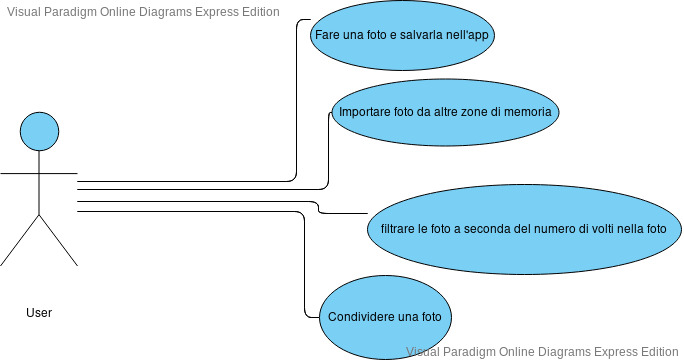
\includegraphics[width=150mm]{images/Use_Case_progetto.jpg}
    \label{fig:my_label}
\end{figure}
\\ L'applicazione ha la seguente struttura logica delle classi che le raggruppa a seconda della loro funzione:
\begin{enumerate}
    \item{Images: \begin{enumerate}
        \item ImagesActivity
        \item ImagesFragment
        \item ImagesPresenter
    \end{enumerate}
    }
    \item{Image Viewer: \begin{enumerate}
        \item ImageViewerActivity
        \item ImageViewerFragment
        \item ImageViewerPresenter
    \end{enumerate}
    }
    \newpage
    \item {Storage:\begin{enumerate}
        \item LocalImageRepository
    \end{enumerate}
    }
    \item{Util: \begin{enumerate}
        \item ImagesAdapter
        \item ImageUtils
        \item ImageViewHolder
        \item MyContext
    \end{enumerate}
    }
    
\end{enumerate}
Più nel dettaglio il class Diagram:

\begin{figure}[h!]
    \begin{center}
    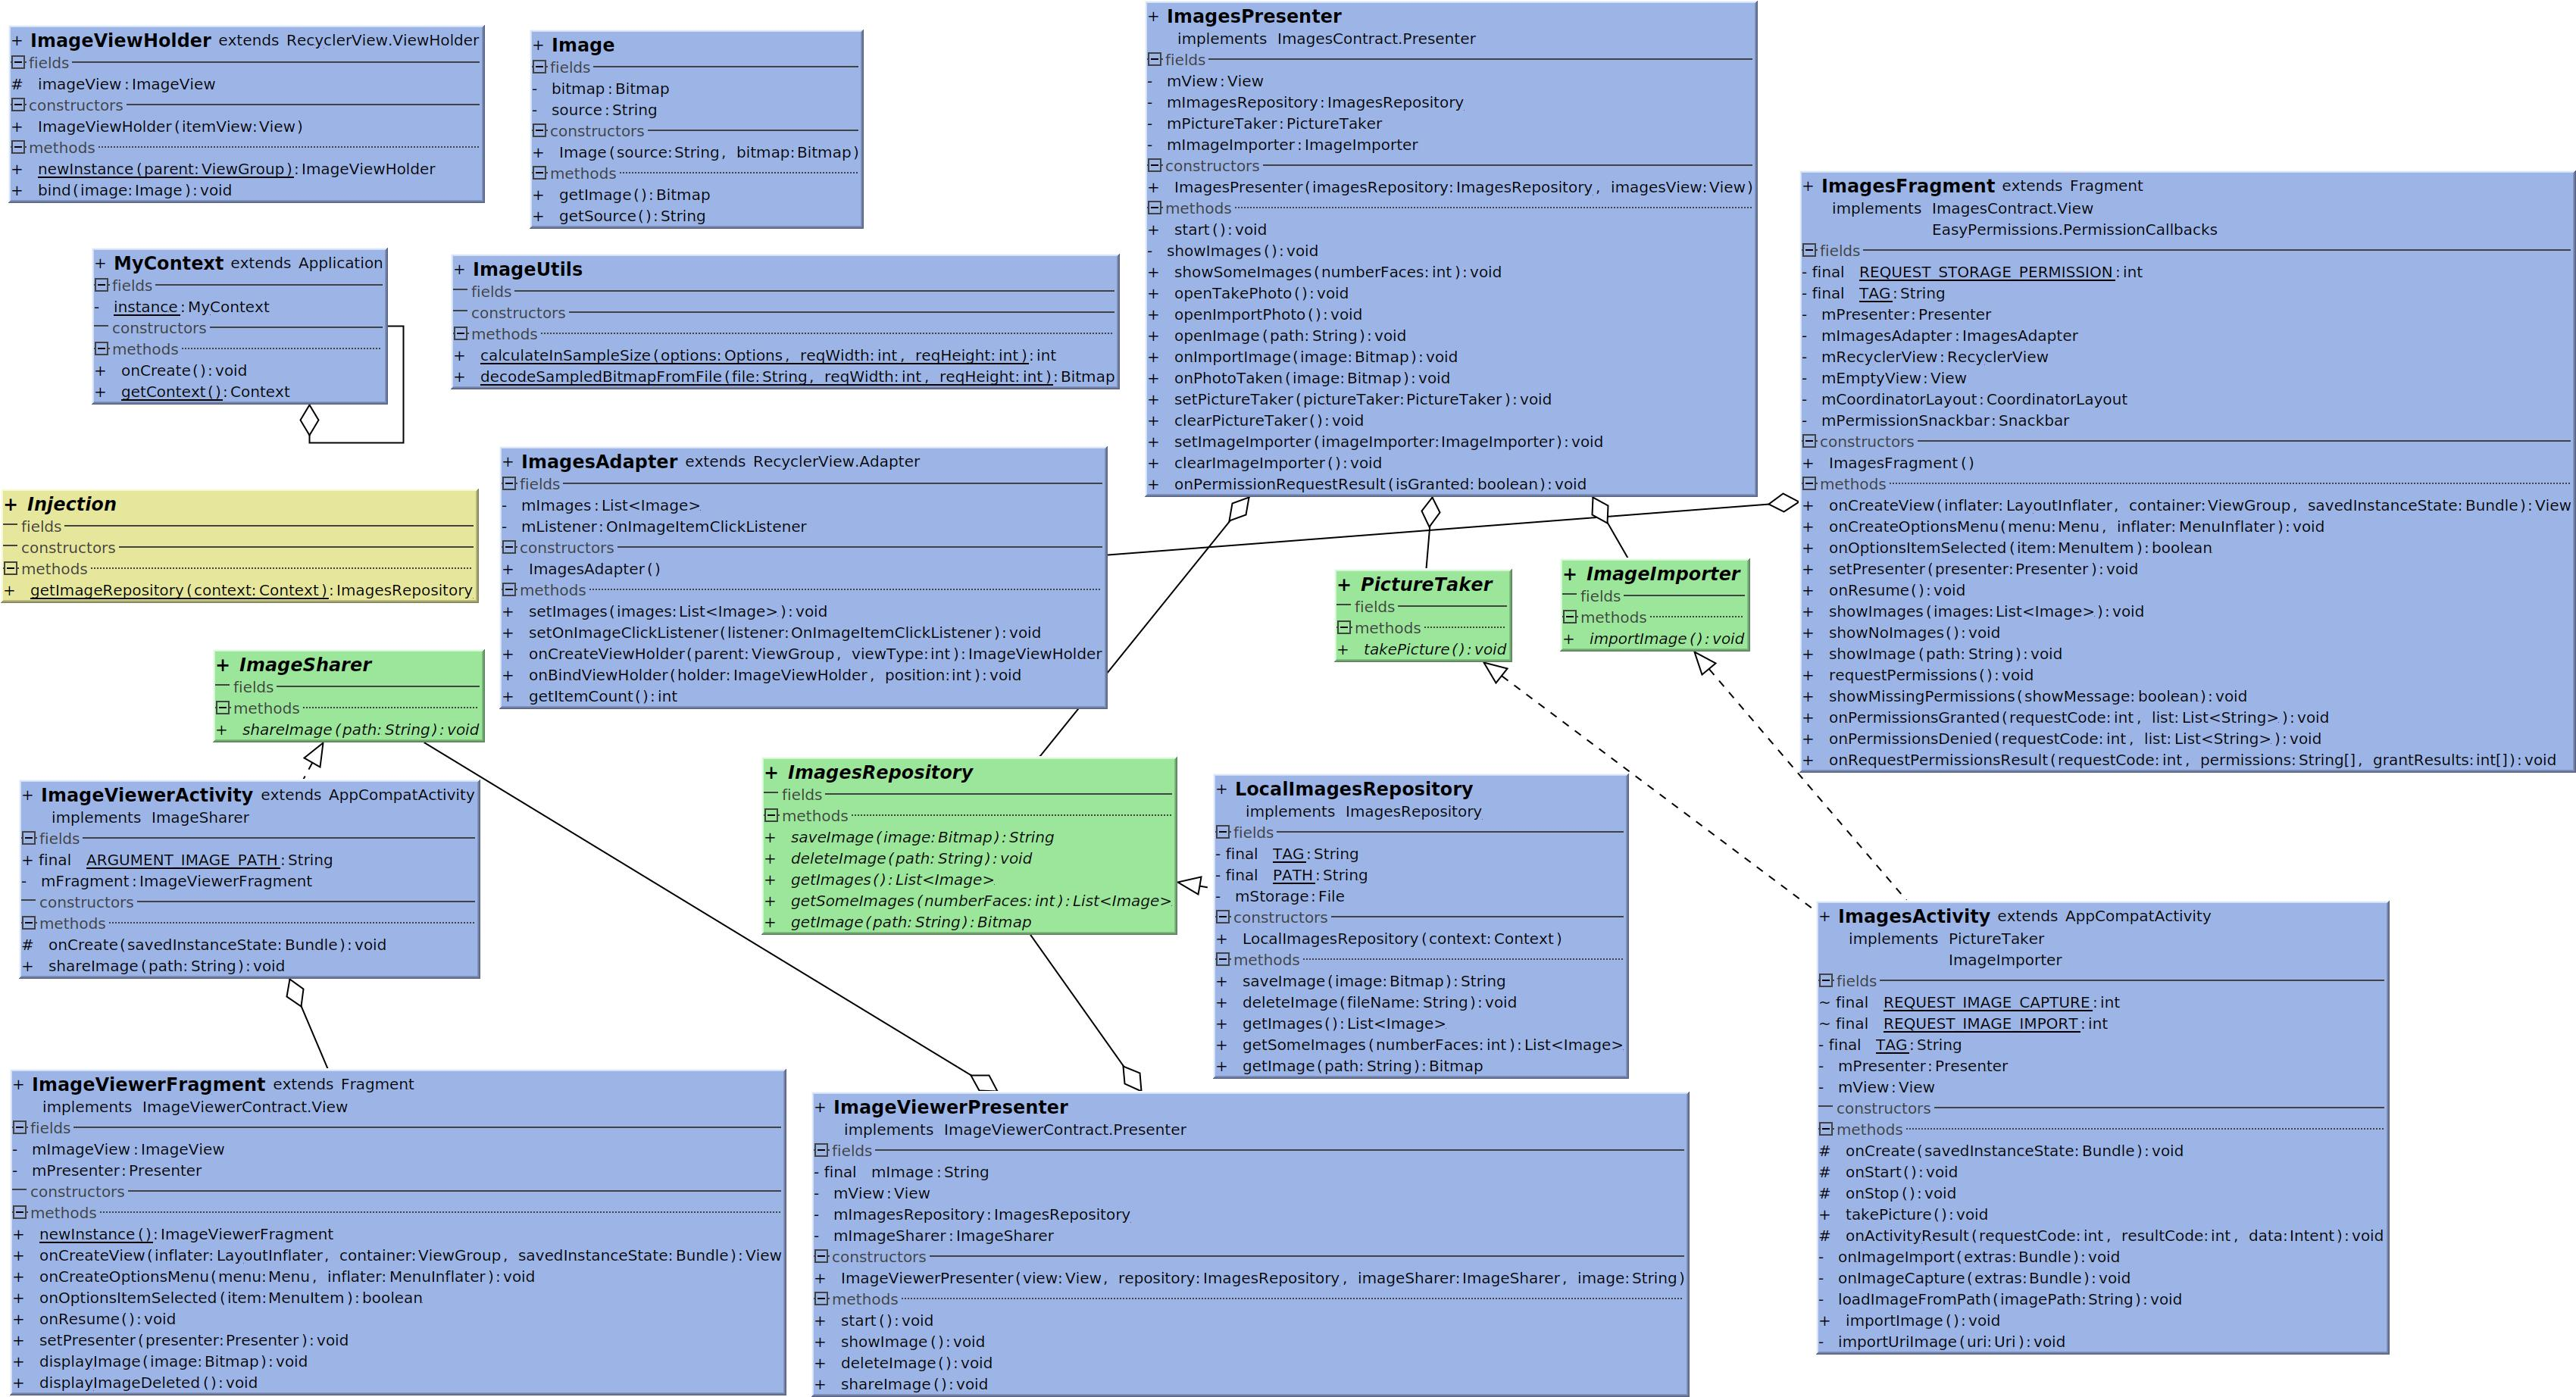
\includegraphics[width=180mm]{images/FINAL CLASS DIAGRAM immagine.jpg}
    \end{center}
\end{figure}

Le classi che ho raggruppato sotto "1. Images" e relative interfacce che vediamo nel class diagramm gestiscono la schermata prinicipale dell'applicazione ovvero quella che vediamo al lancio dell'app.\\
Le classi "2. Image Viewer" gestiscono la seconda schermata dell'app ovvero quella che vediamo quando clicchiamo su un immagine.\\
"3. Storage" gestisce il salvataggio e la memoria dell'applicazione.\\ Infine "4. Util" sono classi necessarie alla gestione generale delle immagini e vengono utilizzate quando necessario dalle altre classi.

\newpage
\section{Scelte progettuali}
Il progetto ha come base di partenza un codelab di google chiamato Keep Sensitive Data Safe and Private. Qui abbiamo quindi la base di partenza per quanto riguarda la struttura delle classi e le scelte iniziali.\\
Inizialmente così si presenta l'applicazione:
\begin{figure}[h!]
  \centering
  \begin{subfigure}
  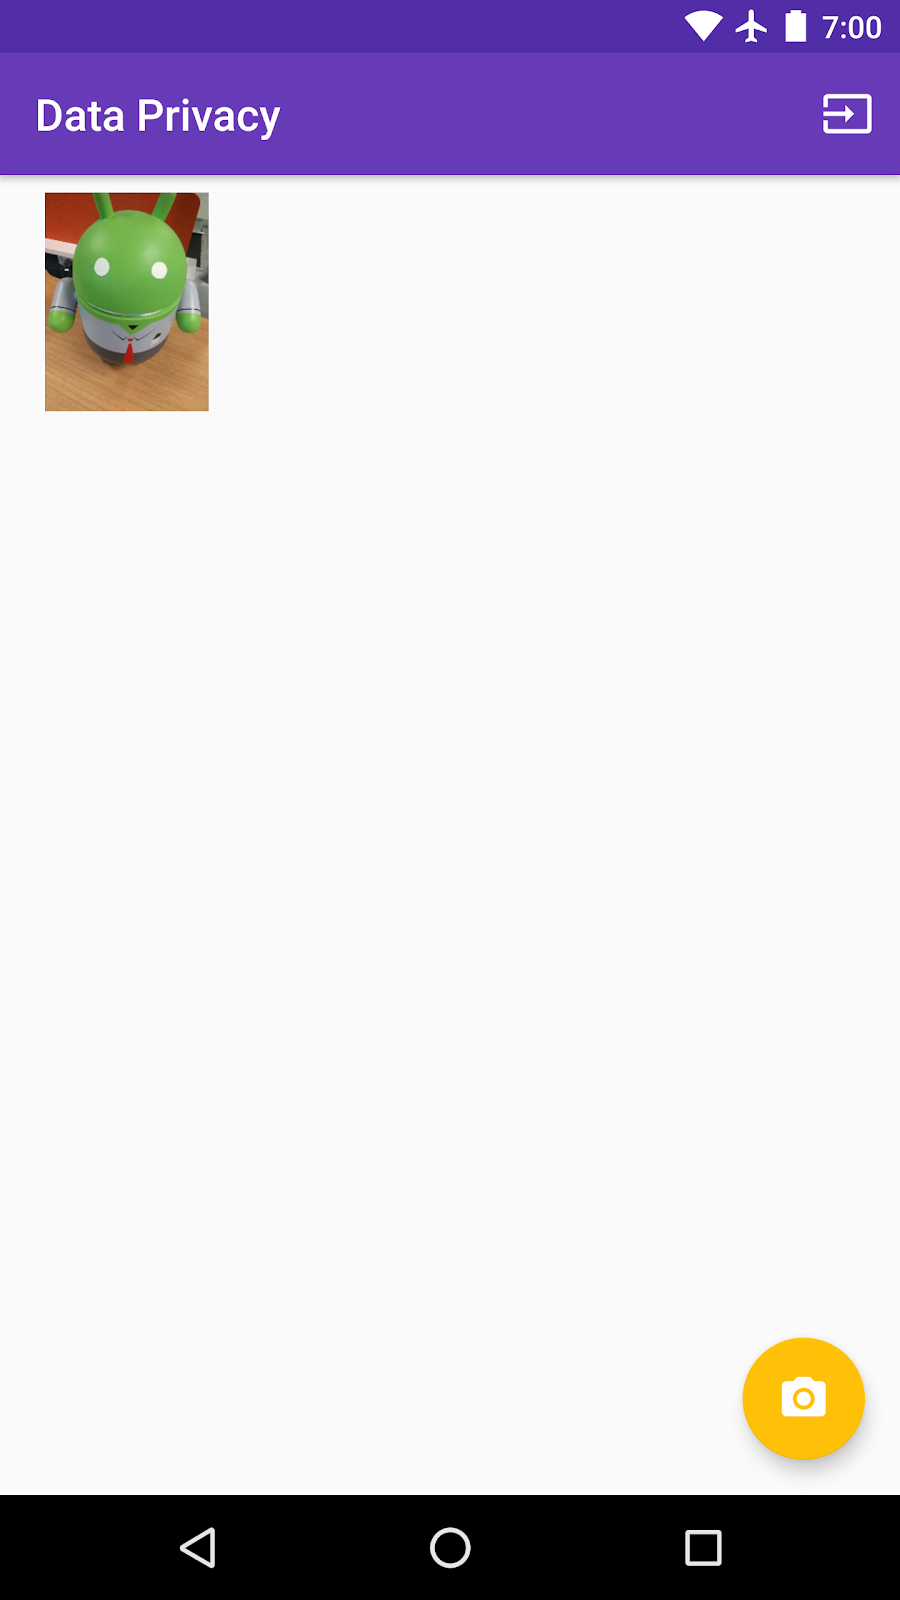
\includegraphics[width=100]{images/Screen1beforecode.png}
  \end{subfigure}
  \begin{subfigure}
  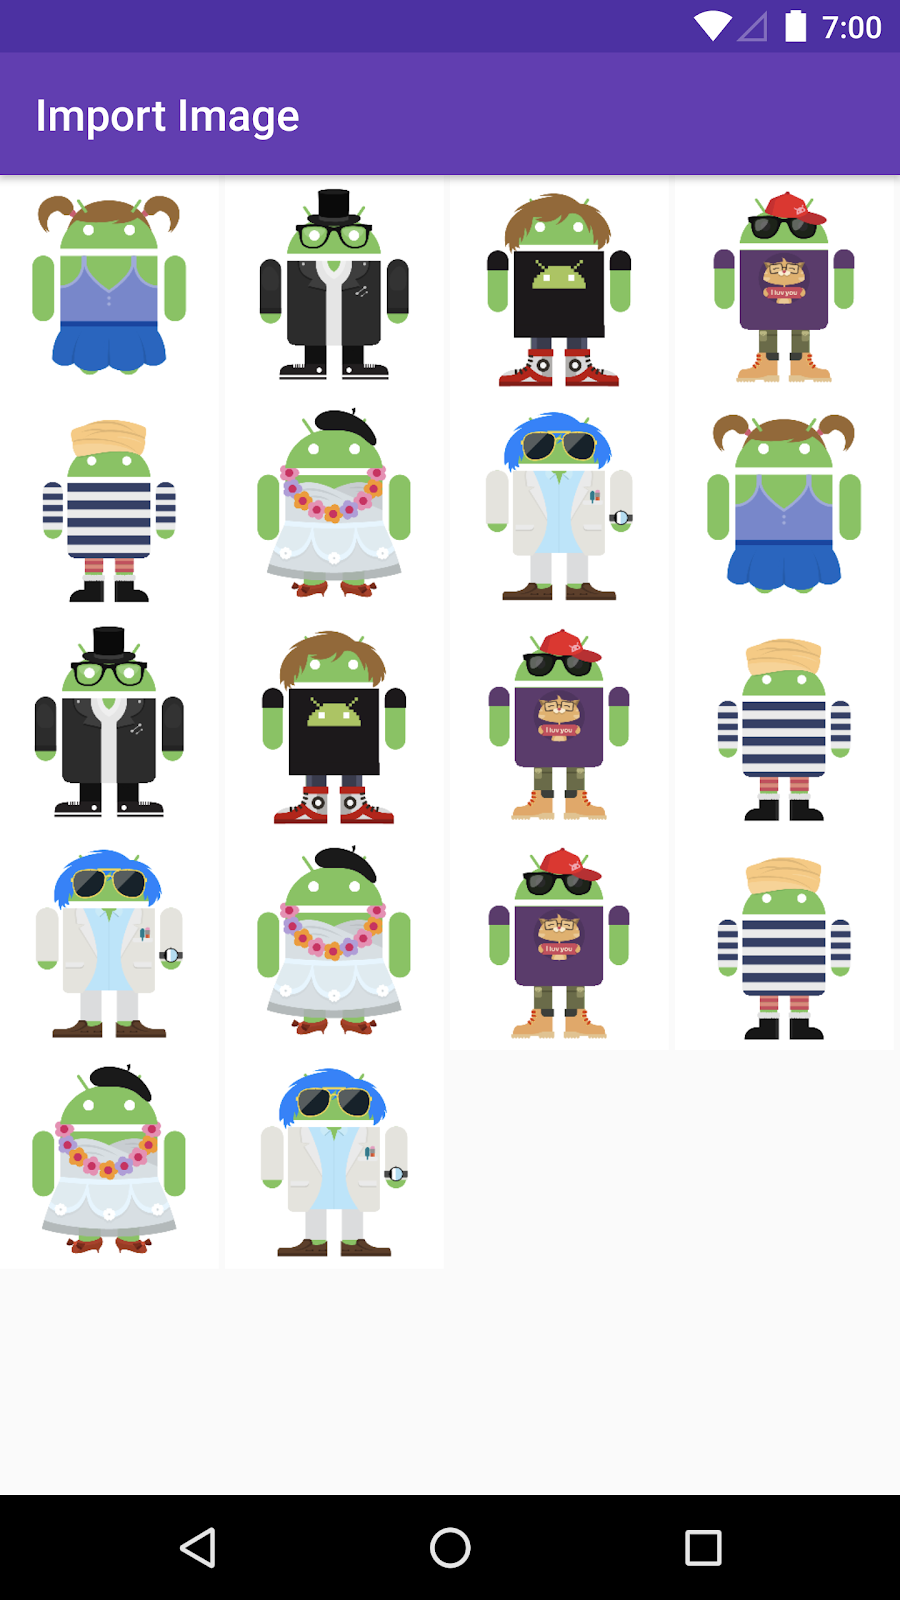
\includegraphics[width=100]{images/Screen2beforecode.png}
  \end{subfigure}
  \begin{subfigure}
    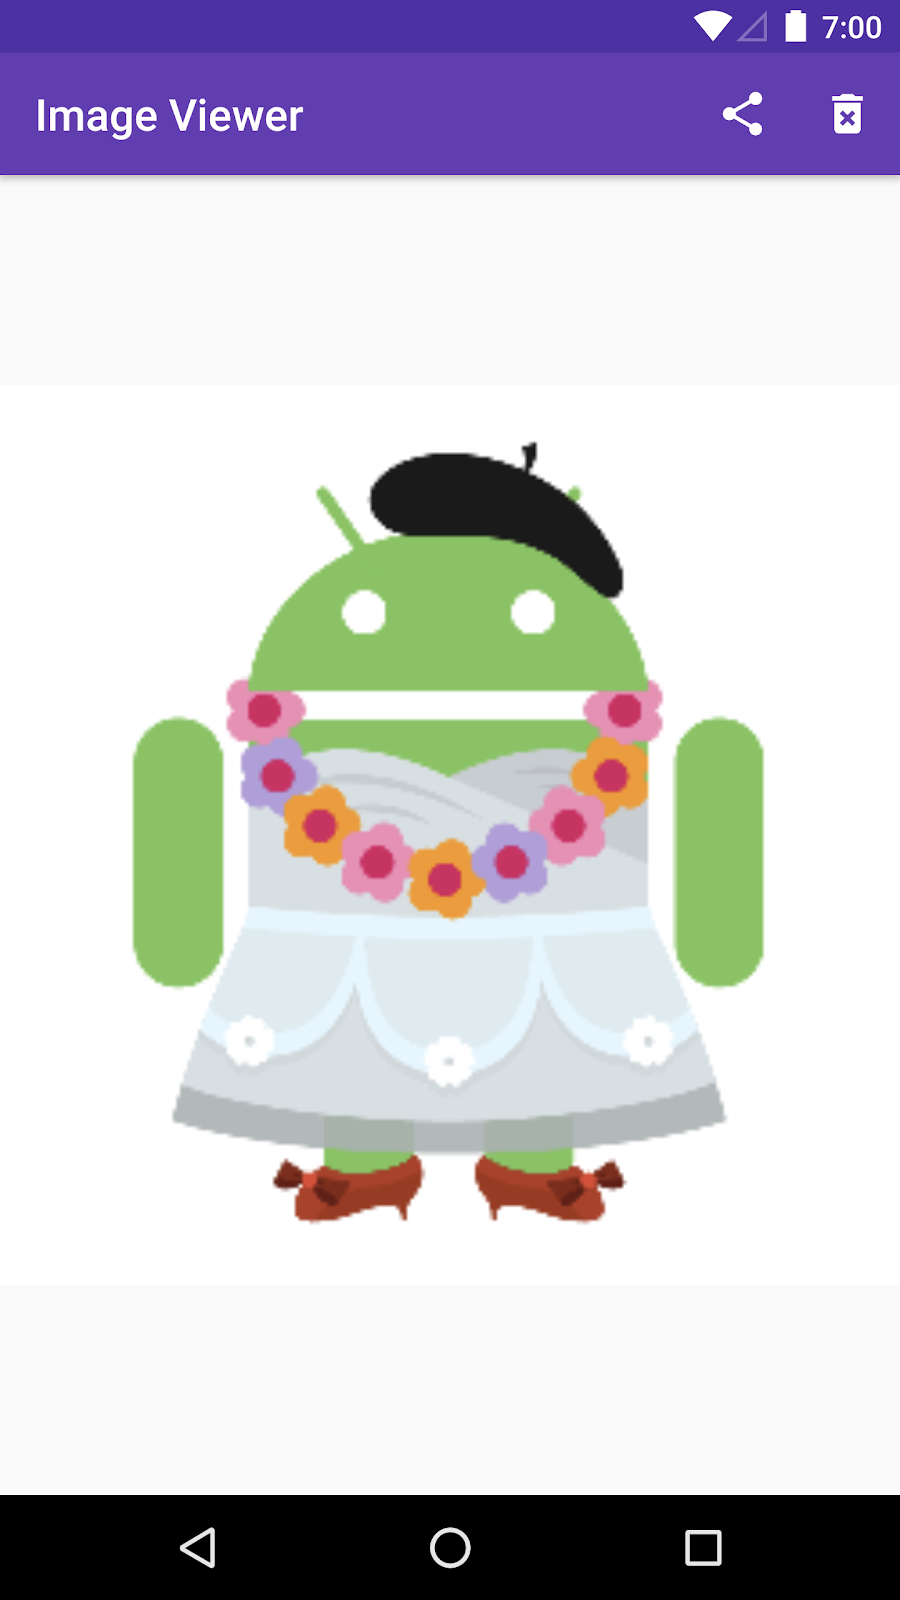
\includegraphics[width=100]{images/Screen3beforecode.png}
  \end{subfigure}
  \label{fig:coffee}
\end{figure}
\subsection{Problemi di sicurezza e Features mancanti}
\begin{enumerate}
    \item Tutte le immagini vengono salvate nella memoria esterna,
    \item Non è implementata la funzione di condivisione delle immagini.
    \item Non è implementata la funzione di identificazione dei volti e nessun modo per filtrare le immagini salvate.
    \item L'applicazione scansiona l'intera memoria esterna per cercare le immagini da importare. Questo viola il prinicipio di minimizzazione dei permessi secondo cui un applicazione NON deve mai richiedere permessi eccessivi. In questo caso il permesso per la memoria esterna.
\end{enumerate}
\subsection{Salvare i dati nella memoria interna}
Ogni applicazione ho una directory di memoria interna privata e non accessibile da altre app e non sono richiesti permessi per accedervi Quando l'utente disinstalla l'app questi file sono rimossi.
Tutto ciò che riguarda il salvataggio dei dati nell'app è gestito dalla classe LocalImagesRepository.
Perciò in questa classe per prima cosa ho rimpiazzato i reference alla memoria esterna con quelli per la memoria interna.\\
Dopodichè ho potuto rimuovere i permessi per scrivere nella memoria esterna nell'AndroidManifest.xml
\subsection{Aggiungere un File Picker Intent}
Ho aggiunto un metodo alla classe ImagesActivity chiamato importImage che viene chiamato quando viene premuta l'icona dell'import sullo schermo. Invece di creare l'Intent e risolverlo all'interno dell'app come è stato implementato inizialmente, il metodo verrà risolto dal sistema.\\
\subsection{Creare un ACTION SHARE Intent per la condivisione}
Ho creato un nuovo metodo in ImageViewerActivity: shareImage(String) usando file providers e content URIs.
\subsection{Facial Detection}
Dovendo scegliere come implementare la funzione che riconosce il numero dei volti nella foto, la scelta fatta è stata quella di aggiungere questo passaggio nel momento in cui si salva la foto nell'applicazione, Aggiungere nel metodo saveImage(Bitmap image) della classe localImageRepository un modo per salvare l'immagine in modo tale che contenesse anche l'informazione del numero di volti presenti. Questo è sembrato il modo migliore per aggiungere tale funzionalità anche per la complessità computazione che questo riconoscimento comporta, in questo modo basta infatti che venga fatto una volta e non ogni volta che voglio filtrare le foto.\\
In particolare ho modificato il modo con cui viene assegnato il file name in modo tale che la prima cifra sia proprio il numero di facce presenti.
\subsubsection{Quali librerie usare}
Dovendo scegliere che librerie usare per fare questo riconoscimento la prima scelta è stata quella di usare le classi ufficiali fornite nelle API per gli Android developers in particolare le classi FaceDetector e Face. Tuttavia testando effettivamente le classi si sono rivelate da subito molto poco performanti e imprecise.
Perciò infine ho deciso di usare le Google APIs for Android, in particolare il pacchetto di Google Cloud Vision, il pacchetto è infatti gratuito per 1-1000 UNITÀ/MESE e qualitativamente è tra i migliori presenti.
\subsection{Filtrare le immagini}
Per quanto riguarda filtrare le immagini ho creato un nuovo metodo nella classe LocalImageRepository: getSomeImages(int numberFaces) e un nuovo metodo nella classe ImagesPresenter: showSomeImages(int numberFaces) che verranno quindi chiamati di volta in volta dalla classe ImagesFragment che gestisce la presentazione delle immagini nell'ImagesActivity tramite un menù a tendina che ho aggiunto.
\newpage
\section{Difficoltà incontrate}
Nello svolgimento del progetto sono state incontrate difficoltà soprattutto iniziali per quanto riguarda l'utilizzo di Android Studio, Gradle e la struttura dell'IDE. Dopodichè nella comprensione della struttura progettuale iniziale del Codelab per capire come intervenire in essa e ha richesto uno studio approfonodito di cosa significa programmare per Android e gestire la UI dell'applicazione quindi capire i cicli di vita di un applicazione, la sintassi XML, la gestione di Views e Layouts, le Activities, i Fragment, i Menù, usare gli Intents, etc.\\
Altre due difficoltà sono state incontrate usando le Google Cloud Vision APIs: La prima perchè la versione più recente delle API creava un errore per la sincronizzazione del progetto con Gradle perchè era fatta per API più recenti di quelle che usava il resto dell'applicazione e l'ho risolto scegliendo una versione più vecchia delle API. La seconda nella scrittura del codice per usarle, infatti per utilizzarle c'è bisogno di creare la classe FaceDetector usando FaceDetector.Builder che però richiede come argomento il context in cui verrà creato il FaceDetector, però nel metodo in cui stavo creando il FaceDetector il context non era passato come argomento, ed ho risolto il problema creando una nuova classe MyContext che permette in ogni luogo dell'applicazione di essere invocata per aver il context.
\section{Considerazioni finali}
Infine posso dire che con questo progetto ho raggiunto un discreto livello per quanto riguarda la programmazione android, ma anche ho imparato a gestire un progetto, usare delle API, e usare vari tool per la risoluzione di problemi. Soprattutto l'esperienza è stata formativa per impare cosa significa davvero nell'atto pratico programmare e usare un linguaggio di programmazione a oggetti come Java.
\end{document}